\begin{figure}[h!]
	\centering
	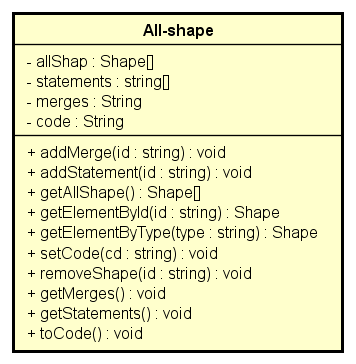
\includegraphics[scale=0.8]{res/sections/SpecificaFrontEnd/Services/Disegnetti/all-shape.png}
	\caption{Diagramma della classe All-shape}
\end{figure}

\begin{itemize}
	\item \textbf{Descrizione:}\\
	
	\item \textbf{Utilizzo:}\\
	
	\item \textbf{Attributi:}
		\begin{itemize}
			\item \emph{-allShap: Shape[]}\\
			
			\item \emph{-statements: string[]}\\
			
			\item \emph{-merges: string}\\
			
			\item \emph{-code: string}\\
			
		\end{itemize}
	\item \textbf{Metodi:}
		\begin{itemize}
			\item \emph{+addMerge(id: string)}\\
    		\\
    		\textbf{Parametri:}
    		\begin{itemize}
    			\item \emph{id: string}\\
    			
    		\end{itemize}
    		\item \emph{+addStatement(id: string)}\\
    		\\
    		\textbf{Parametri:}
    		\begin{itemize}
    			\item \emph{id: string}\\
    			
    		\end{itemize}
    		\item \emph{+getAllShape()}\\
    		
    		\item \emph{+getElementById(id: string)}\\
    		\\
    		\textbf{Parametri:}
    		\begin{itemize}
    			\item \emph{id: string}\\
    			
    		\end{itemize}
    		\item \emph{+getElementByType(type: string)}\\
    		\\
    		\textbf{Parametri:}
    		\begin{itemize}
    			\item \emph{type: string}\\
    			
    		\end{itemize}
    		\item \emph{+setCode(cd: string)}\\
    		\\
    		\textbf{Parametri:}
    		\begin{itemize}
    			\item \emph{cd: string}\\
    			
    		\end{itemize}
    		\item \emph{+removeShape(id: string)}\\
    		\\
    		\textbf{Parametri:}
    		\begin{itemize}
    			\item \emph{id: string}\\
    			
    		\end{itemize}
    		\item \emph{+getMerges()}\\
    		
    		\item \emph{+getStatements()}\\
    		
    		\item \emph{+toCode()}\\
    		
		\end{itemize}
\end{itemize}